\chapter{CP-Verletzung in B-Meson-Systemen}
\section{Diskrete Symmetrietransformationen}
Symmetrien sind in der Physik von zentraler Bedeutung. Gemäß dem Noether-Theorem existiert in der klassischen Physik zu jeder kontinuierlichen Symmetrie eine Erhaltungsgröße. In quantenmechanischen Systemen können wir drei diskrete Symmetrietransformationen betrachten:
\begin{enumerate}
\item \textbf{Parität $\mathcal{P}$:} \\
      Bei der Paritätsoperation wird das Vorzeichen der kartesischen Ortskoordinaten umgekehrt. Dies entspricht einer Punktspigelung.
\item \textbf{Ladungskonjugation $\mathcal{C}$:} \\
      Jedes Teilchen wird durch sein Antiteilchen ersetzt.
\item \textbf{Zeitumkehr $\mathcal{T}$:} \\
      Das Vorzeichen auf der Zeitachse wird umgekehrt. Da in der vorligenden Arbeit allerdings nur die CP-Verletzung gemessen werden soll, wird die Zeitumkehr im folgenden vernachlässigt.
\end{enumerate}
Entgegen der klassischen Intuition konnte Wu 1956 nachweisen, dass die Parität im $\beta$-Zerfall und damit in der schwachen Wechselwirkung nicht erhalten ist. Weitere Experimente zeigen, dass die schwache Wechselwirkung die Parität maximal verletzt: Neutrinos, die nur schwach wechselwirken können, sind stets \glqq linkshändig\grqq (Spin und Impuls antiparallel), Antineutrinos dagegen immer \glqq rechtshändig\grqq (Spin und Impuls parallel). Da der Spin im Gegensatz zum Impuls invariant unter $\mathcal{P}$-Transformation ist, würde diese Operation aus einem linkshändigen Neutrino ein rechtshändiges machen, was in der Nautr nicht realisiert ist.

Damit ist offensichtlich, dass die schwache Wechselwirkung auch die Ladungskonjugation verletzt: Wendet man die $\mathcal{C}$-Transformation auf ein linkshändiges Neutrino an, so erhält man ein linkshändiges Antineutrino. Dieses existiert aber wie bereits erwähnt nicht. Analog gilt die Überlegung auch für Antineutrinos.

\subsection{Scheinbare $\mathcal{CP}$-Invarianz}
Wendet man nun aber die Transformationen $\mathcal{P}$ und $\mathcal{C}$ direkt hintereinander an, so ergibt sich zunächst kein Widerspruch zur Natur (siehe Abb. \ref{fig:cp_invaranz}). Aus einen linkshändigen Neutrino wird ein rechtshändiges Antineutrino. Im Jahre 1964 wurde dann allerdings im Zerfall neutraler K-Mesonen erstmal $\mathcal{CP}$-Verletzung nachgewiesen. \cite{kleinknecht}

\begin{figure}[hptb]
\centering
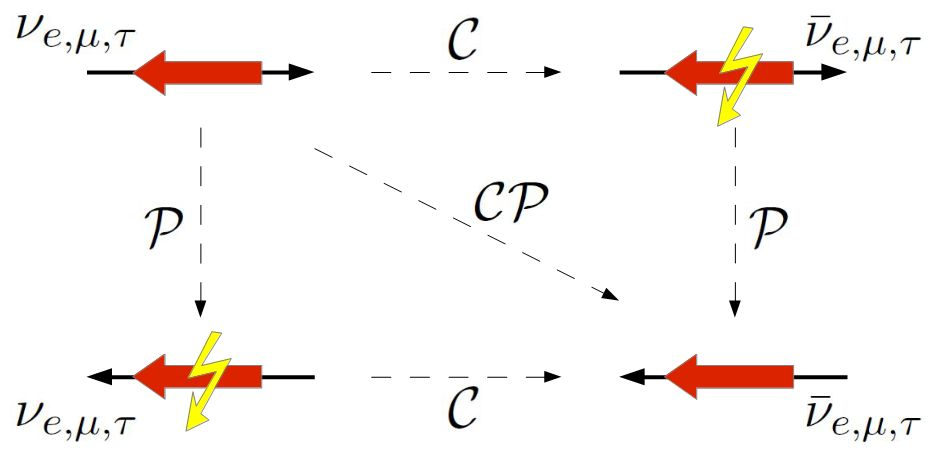
\includegraphics[width = 0.8\textwidth]{cp_invarianz}
\caption{Scheinbare $\mathcal{CP}$-Invarianz: Während eine reine $\mathcal{P}$- oder $\mathcal{C}$-Transformation zu in der Natur nicht realisierten Zuständen führt, scheint es bei der kombinierten $\mathcal{CP}$-Transformation keinen Widerspruch zu geben (dünne Pfeile: Impulsausrichtung, dicke Pfeile: Spinausrichtung).}
\label{fig:cp_invarianz}
\end{figure}



\section{\CP-Verletzung in der Mischung}
Die Flavoureigenzustände $\Ket{B^0} = \Ket{\overline{b}d}$ und $\Ket{\overline{B^0}} = \Ket{b\overline{d}}$ entsprechen nicht den Masseneigenzuständen. Wir definieren daher die normierten Zustände
\begin{align}
\Ket{B_h} = p \Ket{B^0} - q \Ket{\overline{B^0}} \label{eq:b_heavy}\\ 
\Ket{B_l} = p \Ket{B^0} + q \Ket{\overline{B^0}} \label{eq:b_light}\\
\text{mit} \quad |p|^2 + |q|^2 = 1
\end{align}
welche eine definierte Masse und Zerfallsbreite besitzen. Sie sind auch Eigenzustände eines nicht-hermiteschen Hamiltonoperators (Nichthermitizität wegen des möglichen Zerfalls der Teilchens). Dieser setzt sich zusammen aus den hermiteschen Massenoperatoren $M$ und $\Gamma$. Notieren wir die lineare Superposition der Zustände \ref{eq:b_heavy} und \ref{eq:b_light} als $\begin{pmatrix} p \\ q \end{pmatrix}$, so nimmt die zeitabhängige Schrödingergleichung die Form
\begin{align}
\im \diff{}{t}\begin{pmatrix} p \\ q \end{pmatrix} = \left(M - \frac{\im}{2} \Gamma\right) \begin{pmatrix} p \\ q \end{pmatrix}
\end{align}
an und führt zur folgenden zeitlichen Entwicklung der Zustände:
\begin{align}
\nonumber \Ket{B_{h/l}(t)} &= \e^{-\im m_{h/l}t-\frac{1}{2}\Gamma_{h/l}t}\Ket{B_{h/l}(0)} \\
                           &= \e^{-\gamma_{h/l}t}(p\Ket{B^0} \mp q\Ket{\overline{B^0}}) \\
&\text{mit} \quad \gamma_{h/l} = \im m_{h/l}+\frac{\Gamma_{h/l}}{2}
\end{align}
Hierbei ist $\gamma_{h/l}$ so definiert, dass $-\im\gamma_{h/l} = m_{h/l}-\frac{\im}{2}\Gamma_{h/l}$ die Eigenwerte des Hamiltonoperators $\mathcal{H} := \left(M - \frac{\im}{2} \Gamma\right)$ sind. Umgeschrieben auf die Flavoureigenzustände erhalten wir:
\begin{align}
\nonumber \Ket{B^0(t)} &= \frac{1}{2p}\left(\Ket{B_h} + \Ket{B_l}\right) \\
                       &= \frac{1}{2}\left[ (\e^{-\gamma_h t}+\e^{-\gamma_l t})\Ket{B^0} - \frac{q}{p}(\e^{-\gamma_h t}-\e^{-\gamma_l t})\Ket{\overline{B^0}}\right] 
\end{align}
Die Wahrscheinlichkeit für den Übergang eines $\Ket{B^0}$ (zum Zeitpunkt $t=0$) in ein $\Ket{\overline{B^0}}$ beträgt:
\begin{align}
\nonumber P(B^0\rightarrow\overline{B^0})(t) &= |\Braket{\overline{B^0}|B^0(t)}|^2 \\
                                        &= \frac{1}{4} \left|\frac{q}{p}\right|^2 \left[\e^{-\Gamma_h t} + \e^{-\Gamma_l t} - 2\e^{-\frac{1}{2}(\Gamma_h + \Gamma_l) t}\cos(\Delta m_d t)\right] \\
&\text{mit} \quad \Delta m_d = m_h - m_l
\end{align}

\section{Direkte \CP-Verletzung}
Die Zerfallsamplituden der neutralen $B^0$-Mesonen in einen Endzustand $\Ket{f}$ bzw. seinen \CP-konjugierten Zustand $\Ket{\overline{f}}$ sind definiert als
\begin{alignat}{2}
\nonumber A_f &= \Braket{f|\mathcal{H}|B^0}, && \qquad A_{\overline{f}} = \Braket{\overline{f}|\mathcal{H}|B^0}, \\
          \overline{A_f} &= \Braket{f|\mathcal{H}|\overline{B^0}}, && \qquad  \overline{A_{\overline{f}}} = \Braket{\overline{f}|\mathcal{H}|\overline{B^0}}.
\end{alignat}
Dabei bezeichnet $\mathcal{H}$ einen Hamiltonoperator der schwachen Wechselwirkung. Ist \CP erhalten, dann sollten die Zerfallsraten, ergo auch die Zerfallsamplituden eines $B^0$ nach $f$ sowie eines $\overline{B^0}$ nach $\overline{f}$ gleich sein. Dies bedeutet:
\begin{align}
\text{Direkte \CP-Verletzung} \qquad \Longleftrightarrow \qquad \frac{|A_f|}{|\overline{A_{\overline{f}}}|} \neq 1 \quad \text{bzw.} \quad \frac{|\overline{A_f}|}{|A_{\overline{f}}|} \neq 1
\end{align}


\section{\CP-Verletzung in der Interferenz}
